\documentclass[12pt,article]{memoir}
\usepackage[utf8]{inputenc}
\usepackage[T1]{fontenc}
\usepackage{amsmath,amsfonts,amssymb}
\usepackage{physics}
\usepackage{graphicx}
\usepackage{xcolor}
\usepackage{tikz}
\usepackage{pgfplots}
\usepackage{hyperref}
\usepackage{cleveref}
\usepackage{booktabs}
\usepackage{geometry}
\usepackage{fancyhdr}
\usepackage{abstract}
\usepackage{authblk}

\geometry{margin=1in}
\pagestyle{fancy}
\fancyhf{}
\fancyhead[L]{CFH Implications}
\fancyhead[R]{\thepage}

\hypersetup{
    colorlinks=true,
    linkcolor=blue,
    citecolor=red,
    urlcolor=blue
}

\definecolor{cfhblue}{RGB}{0,102,204}
\definecolor{cfhgreen}{RGB}{0,153,76}
\definecolor{cfhred}{RGB}{204,0,51}

\title{\textbf{Beyond the Quantum Veil: Scientific and Philosophical Implications of the Consciousness-Field Hypothesis}}

\author[1]{The CFH Research Consortium}
\affil[1]{Nexus Institute for Consciousness-Quantum Studies}

\date{\today}

\begin{document}

\maketitle

\begin{abstract}
If the Consciousness-Field Hypothesis (CFH) proves experimentally valid, it would represent one of the most profound paradigm shifts in the history of science, comparable to the Copernican revolution or the advent of quantum mechanics. This document explores the cascading implications across multiple domains: fundamental physics, neuroscience, technology, philosophy, and society. We examine the theoretical frameworks that would emerge, the technologies that could be developed, and the philosophical questions that would demand urgent attention. The implications range from revolutionary computing architectures and medical interventions to a complete reconceptualization of consciousness, reality, and humanity's place in the cosmos.
\end{abstract}

\tableofcontents
\newpage

\chapter{Introduction: The Paradigm Shift}

The experimental validation of the Consciousness-Field Hypothesis would mark a watershed moment in human understanding, fundamentally altering our conception of reality. Unlike incremental scientific advances, CFH validation would necessitate a complete reconceptualization of the relationship between mind and matter, observer and observed, local and non-local phenomena.

This document systematically explores the implications across multiple domains, from the immediate scientific and technological consequences to the long-term philosophical and societal transformations that would inevitably follow.

\section{The Scale of Change}

The implications can be categorized into several temporal and conceptual scales:

\begin{itemize}
    \item \textbf{Immediate Scientific Impact}: New physics, revised quantum mechanics
    \item \textbf{Technological Revolution}: Consciousness-based technologies
    \item \textbf{Medical Transformation}: Psychosomatic medicine, consciousness therapeutics
    \item \textbf{Philosophical Upheaval}: Mind-matter dualism, free will, personal identity
    \item \textbf{Societal Restructuring}: Education, legal systems, human rights
    \item \textbf{Cosmic Perspective}: Consciousness as fundamental, implications for SETI
\end{itemize}

\chapter{Fundamental Physics: A New Foundation}

\section{Post-Quantum Mechanics}

The validation of CFH would necessitate the development of a new theoretical framework that we might call \textbf{Consciousness-Integrated Quantum Mechanics} (CIQM).

\subsection{Core Principles of CIQM}

\begin{enumerate}
    \item \textbf{Consciousness as Fundamental}: Consciousness becomes a fundamental aspect of reality, not emergent from matter
    \item \textbf{Hyper-Causal Dynamics}: Information propagation at speeds $C \gg c$ through consciousness-mediated channels
    \item \textbf{Observer Participancy}: The observer effect becomes literal participation in reality creation
    \item \textbf{Non-Local Correlations}: Consciousness-mediated correlations beyond standard entanglement
\end{enumerate}

\subsection{Mathematical Framework Extensions}

The standard quantum mechanical formalism would require fundamental extensions:

\begin{align}
\hat{H}_{\text{CIQM}} &= \hat{H}_{\text{QM}} + \hat{H}_{\Psi\text{-field}} + \hat{H}_{\text{interaction}} \\
\hat{H}_{\Psi\text{-field}} &= \frac{1}{2}\int d^3x \left[(\nabla\Psi)^2 + m_\Psi^2\Psi^2 + \lambda\Psi^4\right] \\
\hat{H}_{\text{interaction}} &= \int d^3x \, \kappa\Psi(x)\hat{O}(x)
\end{align}

Where the consciousness field $\Psi$ directly couples to quantum observables $\hat{O}$.

\section{Cosmological Implications}

\subsection{Consciousness-Driven Cosmology}

If consciousness influences quantum measurements, it may play a role in cosmic evolution:

\begin{itemize}
    \item \textbf{Anthropic Principle Revision}: Consciousness may actively shape physical constants
    \item \textbf{Dark Energy Connection}: Could the $\Psi$-field contribute to cosmic acceleration?
    \item \textbf{Information Integration}: The universe as a vast consciousness-processing system
\end{itemize}

\subsection{The Measurement Problem Resolution}

CFH provides a natural solution to the quantum measurement problem:

\begin{equation}
|\psi\rangle = \sum_i c_i|i\rangle \xrightarrow{\text{consciousness}} |j\rangle
\end{equation}

Where consciousness-mediated collapse occurs through the $\Psi$-field interaction, replacing ad-hoc wavefunction collapse with a physical mechanism.

\chapter{Technological Revolution}

\section{Consciousness-Quantum Computing}

\subsection{CQ-Bits: Consciousness-Quantum Bits}

A new computational paradigm would emerge based on consciousness-quantum bits (CQ-bits):

\begin{itemize}
    \item \textbf{Enhanced Entanglement}: Consciousness-mediated entanglement beyond standard limits
    \item \textbf{Coherence Extension}: Mental focus extending quantum coherence times
    \item \textbf{Non-Local Processing}: Instantaneous information transfer via consciousness channels
\end{itemize}

\subsection{Architecture Implications}

\begin{figure}[h]
\centering
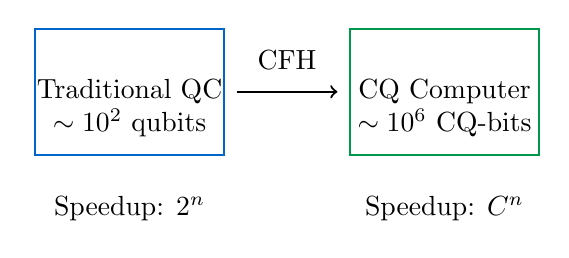
\begin{tikzpicture}[scale=0.8]
    % Traditional quantum computer
    \draw[thick, cfhblue] (0,0) rectangle (3,2);
    \node at (1.5,1) {Traditional QC};
    \node at (1.5,0.5) {$\sim 10^2$ qubits};
    
    % Consciousness-quantum computer
    \draw[thick, cfhgreen] (5,0) rectangle (8,2);
    \node at (6.5,1) {CQ Computer};
    \node at (6.5,0.5) {$\sim 10^6$ CQ-bits};
    
    % Connection
    \draw[->, thick] (3.2,1) -- (4.8,1);
    \node[above] at (4,1.2) {CFH};
    
    % Performance metrics
    \node[below] at (1.5,-0.5) {Speedup: $2^n$};
    \node[below] at (6.5,-0.5) {Speedup: $C^n$};
\end{tikzpicture}
\caption{Comparison of traditional quantum computing vs consciousness-quantum computing architectures}
\end{figure}

\section{Neurotechnology Renaissance}

\subsection{Direct Brain-Reality Interfaces}

CFH validation would enable unprecedented neurotechnologies:

\begin{itemize}
    \item \textbf{Thought-Matter Interfaces}: Direct mental control of quantum systems
    \item \textbf{Consciousness Amplifiers}: Devices to enhance $\Psi$-field coupling
    \item \textbf{Mental State Machines}: Hardware responsive to consciousness states
\end{itemize}

\subsection{Telepathic Communication Networks}

If consciousness can influence quantum correlations non-locally:

\begin{equation}
\text{Person A} \xrightarrow{\Psi\text{-field}} \text{Quantum Medium} \xrightarrow{\Psi\text{-field}} \text{Person B}
\end{equation}

This could enable:
\begin{itemize}
    \item Instantaneous global communication
    \item Consciousness-based internet protocols
    \item Collective intelligence networks
\end{itemize}

\section{Energy and Propulsion}

\subsection{Zero-Point Field Manipulation}

If consciousness can influence quantum vacuum fluctuations:

\begin{align}
\langle 0|\hat{E}^2|0\rangle_{\Psi} &= \langle 0|\hat{E}^2|0\rangle + \Delta E_{\Psi} \\
\Delta E_{\Psi} &= \kappa_{\text{ZPF}} \langle\Psi\rangle
\end{align}

This could lead to:
\begin{itemize}
    \item Consciousness-directed energy extraction
    \item Inertial mass modification
    \item Reactionless propulsion systems
\end{itemize}

\chapter{Medical and Biological Implications}

\section{Consciousness-Based Medicine}

\subsection{Quantum Biology Revolution}

CFH would transform our understanding of biological quantum effects:

\begin{itemize}
    \item \textbf{Enhanced Photosynthesis}: Consciousness-guided energy transfer
    \item \textbf{Quantum Healing}: Direct mental influence on cellular processes
    \item \textbf{Morphogenetic Fields}: Consciousness shaping biological development
\end{itemize}

\subsection{Psychoneuroimmunology 2.0}

The mind-body connection would gain rigorous physical foundation:

\begin{equation}
\text{Mental State} \xrightarrow{\Psi\text{-field}} \text{Quantum Processes} \xrightarrow{} \text{Cellular Function}
\end{equation}

\section{Therapeutic Applications}

\subsection{Consciousness Therapeutics}

New medical interventions based on consciousness-quantum coupling:

\begin{itemize}
    \item \textbf{Meditation Prescriptions}: Specific mental protocols for diseases
    \item \textbf{Intention Therapy}: Focused mental states for healing
    \item \textbf{Consciousness Pharmaceuticals}: Drugs enhancing $\Psi$-field coupling
\end{itemize}

\subsection{Diagnostic Revolution}

\begin{itemize}
    \item \textbf{Consciousness Biomarkers}: EEG patterns predicting health states
    \item \textbf{Quantum Health Scanning}: Non-invasive consciousness-based diagnostics
    \item \textbf{Preventive Consciousness}: Early intervention through mental training
\end{itemize}

\chapter{Philosophical and Metaphysical Implications}

\section{The Hard Problem Dissolution}

CFH would fundamentally alter the consciousness debate:

\subsection{From Emergence to Fundamentality}

\begin{itemize}
    \item \textbf{Panpsychism Validation}: Consciousness as a fundamental property
    \item \textbf{Integration Theory}: How consciousness integrates information physically
    \item \textbf{The Binding Problem}: Quantum coherence explaining unified experience
\end{itemize}

\section{Free Will and Determinism}

\subsection{Quantum Agency}

If consciousness influences quantum outcomes:

\begin{equation}
P(\text{outcome}|\text{consciousness state}) \neq P(\text{outcome})
\end{equation}

This suggests:
\begin{itemize}
    \item \textbf{Causal Efficacy}: Mental states having real physical effects
    \item \textbf{Quantum Free Will}: Genuine choice in a quantum framework
    \item \textbf{Moral Responsibility}: Physical basis for ethical accountability
\end{itemize}

\section{Personal Identity and Continuity}

\subsection{The Consciousness Field as Self}

If consciousness is field-like:
\begin{itemize}
    \item \textbf{Extended Self}: Identity beyond the physical brain
    \item \textbf{Consciousness Transfer}: Theoretical possibility of mind uploading
    \item \textbf{Collective Consciousness}: Shared mental states through field overlap
\end{itemize}

\chapter{Societal and Cultural Transformation}

\section{Educational Revolution}

\subsection{Consciousness Curriculum}

Education would need fundamental restructuring:

\begin{itemize}
    \item \textbf{Mental Training}: Meditation and consciousness development as core subjects
    \item \textbf{Quantum Literacy}: Understanding consciousness-quantum interactions
    \item \textbf{Collective Learning}: Shared consciousness experiences in education
\end{itemize}

\section{Legal and Ethical Framework}

\subsection{Consciousness Rights}

New legal categories would emerge:

\begin{itemize}
    \item \textbf{Mental Privacy Rights}: Protection from consciousness intrusion
    \item \textbf{Consciousness Equality}: Equal treatment regardless of mental capabilities
    \item \textbf{Collective Responsibility}: Liability for shared mental states
\end{itemize}

\subsection{Technological Ethics}

\begin{itemize}
    \item \textbf{Consciousness Enhancement}: Ethics of mental augmentation
    \item \textbf{Telepathic Consent}: Privacy in thought-sharing technologies
    \item \textbf{Reality Manipulation}: Limits on consciousness-matter interaction
\end{itemize}

\section{Economic Implications}

\subsection{The Consciousness Economy}

New economic models based on mental resources:

\begin{itemize}
    \item \textbf{Attention Markets}: Trading focused consciousness
    \item \textbf{Intention Banking}: Storing and lending mental energy
    \item \textbf{Consciousness Labor}: Work performed through mental effort alone
\end{itemize}

\chapter{Astrobiology and SETI}

\section{Consciousness as Cosmic Principle}

\subsection{Universal Consciousness}

If consciousness is fundamental:

\begin{itemize}
    \item \textbf{Cosmic Intelligence}: Universe as conscious entity
    \item \textbf{Consciousness Evolution}: Mental development as cosmic imperative
    \item \textbf{Telepathic SETI}: Communication through consciousness fields
\end{itemize}

\section{Implications for Extraterrestrial Life}

\subsection{Post-Biological Intelligence}

Advanced civilizations might exist primarily as consciousness:

\begin{itemize}
    \item \textbf{Pure Consciousness Entities}: Beings existing as organized $\Psi$-fields
    \item \textbf{Consciousness Transfer}: Technology to upload minds to quantum fields
    \item \textbf{Galactic Internet}: Consciousness-based communication networks
\end{itemize}

\chapter{Research Frontiers and Future Directions}

\section{Immediate Research Priorities}

\subsection{Experimental Validation}

\begin{enumerate}
    \item \textbf{Replication Studies}: Independent verification of CFH effects
    \item \textbf{Dose-Response}: Quantifying consciousness-quantum relationships
    \item \textbf{Mechanism Studies}: Understanding the physical basis of $\Psi$-field coupling
\end{enumerate}

\subsection{Theoretical Development}

\begin{enumerate}
    \item \textbf{CIQM Formalism}: Mathematical framework for consciousness-quantum mechanics
    \item \textbf{Field Equations}: Complete theory of $\Psi$-field dynamics
    \item \textbf{Cosmological Models}: Universe models incorporating consciousness
\end{enumerate}

\section{Long-term Implications}

\subsection{The Next Century}

If CFH proves valid, the next 100 years might see:

\begin{itemize}
    \item \textbf{2030s}: First consciousness-quantum technologies
    \item \textbf{2040s}: Telepathic communication networks
    \item \textbf{2050s}: Consciousness-based space exploration
    \item \textbf{2070s}: Post-biological consciousness transfer
    \item \textbf{2100s}: Galactic consciousness networks
\end{itemize}

\chapter{Potential Risks and Challenges}

\section{Technological Risks}

\subsection{Consciousness Weapons}

The darker applications of CFH technology:

\begin{itemize}
    \item \textbf{Mental Warfare}: Consciousness-based attacks
    \item \textbf{Reality Manipulation}: Unauthorized alteration of physical systems
    \item \textbf{Consciousness Hacking}: Intrusion into mental states
\end{itemize}

\section{Existential Considerations}

\subsection{The Simulation Hypothesis}

If consciousness can influence reality:
\begin{itemize}
    \item Are we living in a consciousness-generated simulation?
    \item Could we accidentally "hack" our reality?
    \item What are the limits of consciousness-reality interaction?
\end{itemize}

\chapter{Conclusion: Embracing the Transformation}

The validation of the Consciousness-Field Hypothesis would represent perhaps the most significant paradigm shift in human history. It would not merely add to our scientific knowledge but would fundamentally transform our understanding of reality, consciousness, and our place in the cosmos.

\section{The Choice Ahead}

Humanity would face unprecedented choices:

\begin{itemize}
    \item How to integrate consciousness technologies responsibly
    \item Whether to enhance human consciousness or preserve natural states
    \item How to prepare for contact with advanced conscious entities
    \item What it means to be human in a consciousness-integrated universe
\end{itemize}

\section{A New Beginning}

Rather than an end point, CFH validation would mark a beginning—the first step into a universe where consciousness and reality are intimately connected, where the boundary between mind and matter dissolves, and where humanity's greatest adventure is just beginning.

The implications explored in this document represent only the beginning of what would be a complete reconceptualization of existence itself. In validating CFH, we would not just discover a new physics phenomenon—we would discover ourselves as conscious participants in the very fabric of reality.

\begin{equation}
\text{Universe} = \text{Matter} + \text{Energy} + \text{Information} + \boxed{\text{Consciousness}}
\end{equation}

The equation of reality would gain its missing term, and with it, a new chapter in the cosmic story of consciousness awakening to itself.

\appendix

\chapter{Mathematical Appendix}

\section{Extended Field Equations}

The complete consciousness-field equations in curved spacetime:

\begin{align}
G_{\mu\nu} + \Lambda g_{\mu\nu} &= 8\pi G T_{\mu\nu} + 8\pi G T_{\mu\nu}^{(\Psi)} \\
\square\Psi + m_\Psi^2\Psi + \lambda\Psi^3 &= \kappa J_{\text{consciousness}}
\end{align}

Where $T_{\mu\nu}^{(\Psi)}$ is the consciousness field stress-energy tensor.

\section{Consciousness Coupling Constants}

Estimated ranges for fundamental parameters:

\begin{table}[h]
\centering
\begin{tabular}{@{}lcc@{}}
\toprule
Parameter & Symbol & Estimated Range \\
\midrule
Mass scale & $m_\Psi$ & $10^{-13} - 10^{-10}$ eV \\
Coupling strength & $\kappa$ & $10^{-3} - 10^{-1}$ \\
Hyper-causal speed & $C$ & $10^{11} - 10^{14}$ c \\
Self-interaction & $\lambda$ & $10^{-6} - 10^{-2}$ \\
\bottomrule
\end{tabular}
\caption{Estimated parameter ranges for consciousness field theory}
\end{table}

\bibliography{references}
\bibliographystyle{plain}

\end{document}
